\setchapterpreamble[u]{\margintoc}
\chapter{Artificial Atomization : The Falling Raindrop}
\labch{raindrop}

A flow configuration that combines the complexities of large 
density-ratios with the interaction between capillary, viscous and 
inertial stresses is that of a water droplet falling in the 
air under the influence of gravitational acceleration. 

%---------------------------------------------------------------
\section{Problem Setup}

The problem is characterized by a combination of Reynolds, 
Weber and Bond numbers, the definitions of which are as follows : 

\begin{align}
We=\frac{\rho_{g} U^2 D}{\sigma} \quad,\quad Re= \frac{\rho_{l} U D}{\mu_{g}} \quad,\quad Bo=\frac{\left(\rho_{l}-\rho_{g}\right) g D^2 }{\sigma}
\end{align}

The subscripts $l$ and $g$ represent liquid and gas phases respectively. 
In our particular numerical setup, $We \simeq 3.2 $, $Re \simeq 1455 $ and $Bo \simeq 1.2 $, 
thus corresponding to that of a $3mm$ diameter raindrop (a relatively large one) 
falling in the air at an approximate terminal velocity of  
$8$ m/s (interpolated from empirical data, refer to Gunn and Kinzer \cite{gunn1949}). 
The parameters in the problem setup are given in Table \ref{raindropprop}, 
and the schematic diagram given in Fig. \ref{setup}. 
The droplet is initially placed at the center of a cubic domain (3D), 
whose side is 4 times the diameter of the drop. 

\begin{table*}[h!]
\begin{center}
\begin{tabular}{ccccccc}
\hline\hline
$\rho_{g}$ & $\rho_{l}$ & $\mu_{g}$ 
& $\mu_{l}$ & $\sigma$ & $D$ & $g$\\
$\left(kg/m^3\right)$ & $\left(kg/m^3\right)$ & $\left(Pa \, s\right)$ 
& $\left(Pa \,s \right)$ & $\left(N/m\right)$ & $(m)$ & $(m /s^{2})$ \\
\hline
1.2 & $0.9982 \times 10^3$ & $1.98 \times 10^{-5}$ & 
$8.9 \times 10^{-4}$ & $0.0728$ & $3 \times 10^{-3}$ & $9.81$\\
\hline\hline
\end{tabular}
\caption{Parameter values used in the simulation 
	of a falling water droplet in air. \label{raindropprop}}
\end{center}
\end{table*}


In order to properly reproduce and analyse the dynamics 
of a relatively large drop (high Reynolds flow) such as in our case, 
the numerical method has to accurately resolve the thin boundary layers, 
the interaction of such layers with the capillary forces and finally 
the non-linear feedback of the complex 
3D vortical structures present in the wake behind the droplet. 
Such an undertaking was attempted by Dodd and Ferrante \cite{dodd2014}, 
in which they managed to delineate the different regimes concerning the 
behavior of the wake behind the droplet, although at relatively 
lower Reynolds numbers (the maximum Reynolds tested was $\simeq 500$, 
whereas in our case it is $\simeq 1500$).    
Therefore, our objective behind the demonstration of this particular 
test case is \textit{not} to develop a high fidelity model of a raindrop, 
but rather carry out a stringent evaluation of the robustness of our numerical 
method compared to ones that are not mass-momentum consistent. 
For such a low Weber number the capillary forces dominate and the 
droplet should remain intact, and definitely not undergo any subsequent atomization. 


% -----
\begin{figure}[h!]
\begin{center}
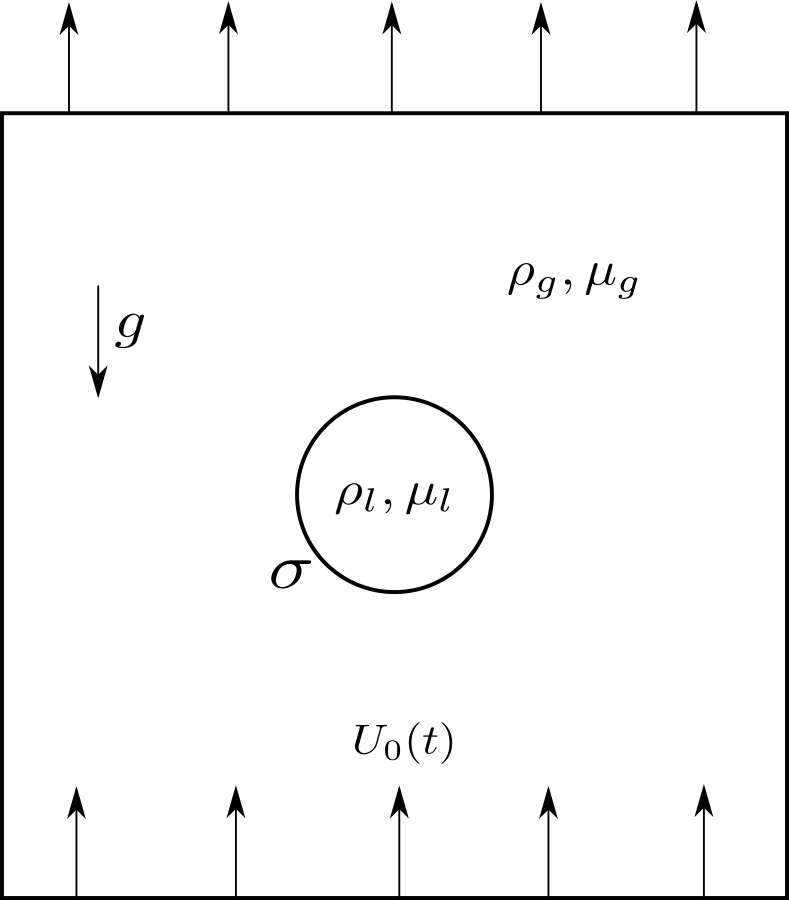
\includegraphics[width=0.5\textwidth]{plots/raindrop/setup.png}
\end{center}
\caption{A 2D schematic of the numerical setup for the falling raindrop. 
	A droplet of diameter $D$ is placed at the center of a cubic domain 
	of side $L$ and $L/D = 4$. The liquid properties ($\rho_l$ , $\mu_l$) 
	correspond to that of water, and the gas properties ($\rho_g$,$\mu_g$) 
	correspond to that of air. We apply a uniform inflow velocity condition 
	with $U_0(t)$ and an outflow velocity condition at the top which 
	corresponds to zero normal gradient.
	Boundary conditions on the side walls correspond 
	to those of impenetrable free slip (no shear stress).}
\label{setup}
\end{figure}

%---------------------------------------------------------------
\section{Numerical Instabilities}

Numerical simulations of this test case at moderate resolution 
(from $D/h=16$ to $D/h=64$) carried out \textit{without} the 
consistent scheme described in this paper results in the catastrophic 
deformations of the droplet as illustrated in Fig. \ref{cata}, 
which we describe as `fictitious' or `artificial' atomization. 
We propose the following explanation in order to account for such numerical artifacts. 
To start with, we neglect gravity and viscous effects at this relatively large Reynolds number. 
Also, we are interested in steady-state flow. 
On the axis and near the hyperbolic stagnation point 
at the front of the droplet one has $u_2=0$ for the transverse 
(radial) velocity and for the axial momentum balance


\begin{align}
u_1 \partial_1 u_1 = - \frac 1 \rho \partial_1 p.
\end{align}

Due to the large viscosity and density ratios, it is not possible for 
the air flow to immediately entrain the water, so the fluid velocity 
is significantly smaller inside the droplet. 
In the air the acceleration near the stagnation point is 
of the order $U^2/D$, whereas the pressure gradient is

\begin{align}
\partial_1 p \sim \rho_{g} U^2/D.
\end{align}
The pressure gradient in the water is much smaller, 
however, in the case of a mixed cell the water density 
multiplies the air acceleration $U^2/D$, so that

\begin{align}
\partial_1 p \sim \rho_{l} U^2/D,
\end{align}

then a large pressure gradient results in the mixed cell or cells. 
This large pressure gradient results in a large pressure inside the 
droplet near the front stagnation point, as shown in Figure \ref{pressure_1}. 
This large pressure is balanced by surface tension only for a sufficiently 
large curvature near the droplet front. 
This explains the presence of a ``dimple'' often observed in low 
resolution simulations of the falling drop. 
This artifact had been observed by Xiao \cite{xiao2012} in a similar case 
involving the sudden interaction of a droplet at rest with a uniform gas flow. 
The resulting large un-physical pressure gradients across the interface 
eventually lead to its rapid destabilization and concomitant breakup.  



%---------------------------------------------------------------

\section{Effect of Mass-Momentum Consistent Transport}



